\chapter{Extensiones posteriores a la estimación}
\label{chap:anexo-extensiones}

Este anexo reúne el detalle de las ocho extensiones que la Sección~\ref{sec:extensiones} resume: seis no preespecificadas, propuestas por revisiones posteriores a la estimación, y dos con preregistro (los bancos como unidad de análisis y los umbrales de vigilancia). Cada una se reporta con su resultado, sea cual sea.

\section{A frecuencia mensual, la fragilidad antecede al spread}
\label{sec:mensual}

Con datos trimestrales, la fragilidad y el spread se mueven dentro del mismo trimestre y no se puede ordenar qué ocurre primero (Sección~\ref{sec:estacionariedad}). Por eso las dos series se construyeron por mes. La fragilidad es menos la distancia al incumplimiento media del sistema ($-DD_w$; Sección~\ref{sec:robustez}), calculada con el mismo motor y los mismos bancos que $JLoss$: la capitalización del último día del mes, la volatilidad realizada de los últimos tres meses y el balance más reciente. No se calcula $JLoss$ mensual porque satura, y la distancia al incumplimiento lleva su misma señal (correlación de $0{,}85$). El spread es el EMBI diario, promediado en los últimos cinco días hábiles de cada mes. La serie mensual reproduce la trimestral en los meses de cierre de trimestre (correlación de $0{,}9993$). El panel tiene 2\,655 país-meses de las trece economías, con efectos fijos de país y de mes.

\begin{table}[htbp]
\centering
\small
\caption[Fragilidad y spread mensuales]{Fragilidad y spread a frecuencia mensual: qué antecede a qué}
\label{tab:mensual}
\begin{adjustbox}{max width=\linewidth}
\begin{tabular}{l cc}
\toprule
 & Coeficiente & $p$ \\
\midrule
\multicolumn{3}{l}{\textit{A. La fragilidad antecede al spread: $\Delta\ln$ EMBI$_m$ sobre $\Delta(-DD_w)_{m-k}$, $k=1,2,3$}} \\
\quad Rezago de un mes & $0{,}013^{***}$ & DK $0{,}005$ \\
\quad Suma de los tres rezagos & $0{,}027^{**}$ & DK $0{,}017$; \textit{cluster} $0{,}001$ \\
\quad Wald conjunto & & DK $0{,}038$; \textit{wild} $<0{,}001$ \\
\quad Sin cada país: suma (rango) & $[0{,}016;\,0{,}033]$ & rezago de un mes $<0{,}05$ en 13 de 13 \\
\addlinespace
\multicolumn{3}{l}{\textit{B. El spread no antecede a la fragilidad: $\Delta(-DD_w)_m$ sobre $\Delta\ln$ EMBI$_{m-k}$}} \\
\quad Suma de los tres rezagos; Wald conjunto & $0{,}029$ & DK $0{,}87$ / $0{,}29$; \textit{wild} $0{,}39$ \\
\addlinespace
\multicolumn{3}{l}{\textit{C. Asociación en el mismo mes y respuesta acumulada}} \\
\quad Mismo mes & $0{,}020^{***}$ & DK $0{,}002$; \textit{wild} $0{,}001$ \\
\quad Respuesta acumulada a 1 / 3 / 6 meses & $0{,}021$ / $0{,}027$ / $0{,}014$ & $0{,}005$ / $0{,}001$ / $0{,}08$ \\
\addlinespace
País-meses (economías) & \multicolumn{2}{l}{2\,655 (13); 2\,603 en el panel A} \\
\bottomrule
\end{tabular}
\end{adjustbox}
\par\smallskip\parbox{0.95\linewidth}{\footnotesize \textit{Nota:} $DD_w$: distancia al incumplimiento de Merton media ponderada por pasivos, mensual; EMBI: promedio de los últimos cinco días hábiles del mes. Paneles A y B: tres rezagos de cada diferencia, efectos fijos de país y de mes, Driscoll--Kraay con seis rezagos; \textit{wild cluster bootstrap} por país con pesos de Webb y 999 réplicas. Panel C: proyecciones locales de $\ln$ EMBI$_{m+h}-\ln$ EMBI$_{m-1}$ sobre $\Delta(-DD_w)_m$ con los mismos controles. Fuente: \texttt{p37\_mensual\_fechado.py}.}
\end{table}

La Tabla~\ref{tab:mensual} muestra que, a frecuencia mensual, la fragilidad sí antecede al spread. Un aumento de la fragilidad en un mes va seguido de un spread mayor en el siguiente ($0{,}013$; $p=0{,}005$), y la suma de los tres rezagos es significativa con los tres métodos de inferencia y sin cada una de las trece economías. En la dirección inversa no hay nada: el spread pasado no anticipa la fragilidad ($p$ de \textit{wild bootstrap} de $0{,}39$). La magnitud es pequeña: una desviación estándar del cambio mensual de la fragilidad ($0{,}43$) va seguida de un spread un $0{,}6\%$ mayor el mes siguiente y un $1{,}2\%$ mayor acumulado a tres meses. La conclusión trimestral de que la fragilidad no antecede al spread era, por tanto, una limitación de la frecuencia: dentro del trimestre, la fragilidad se mueve primero. Sigue siendo una precedencia estadística y no un efecto causal, porque los precios accionarios de los bancos pueden incorporar antes la misma información que después recoge el spread.

\section{Un instrumento granular para la fragilidad}
\label{sec:giv}

Las variables instrumentales de la Sección~\ref{sec:identificacion} usan choques globales con exposiciones previas. Un instrumento propiamente bancario es el granular de \citet{GabaixKoijen2024}. En cada economía y trimestre se toma el retorno accionario de los bancos ponderado por su participación en los pasivos del sistema, menos el de igual ponderación. Todo choque común a los bancos de un país, incluida una noticia soberana que los afecte por igual, se cancela en la diferencia, y queda la parte idiosincrásica de los bancos grandes, que mueve la fragilidad del sistema por su peso.

El instrumento es débil. En la primera etapa, el estadístico $F$ es de $1{,}8$ con Driscoll--Kraay y de $3{,}2$ con errores agrupados para $\ln JLoss$, y de $1{,}9$ y $3{,}0$ para la distancia al incumplimiento; la forma reducida, que con un instrumento es la prueba de Anderson--Rubin, no se distingue de cero ($p$ de \textit{wild bootstrap} de $0{,}81$). La estimación por mínimos cuadrados en dos etapas coincide en punto con la de mínimos cuadrados ordinarios ($0{,}107$ frente a $0{,}104$), pero con un error estándar tres veces mayor ($0{,}36$). Además, la exclusión es dudosa: el instrumento responde al cambio del spread del mismo trimestre ($p=0{,}041$), como ocurriría si los bancos grandes tuvieran una exposición soberana distinta de la de los chicos. Con sistemas de tres a diez bancos cotizados, la parte granular es demasiado pequeña para identificar. El instrumento queda como una vía para un panel con más bancos por economía.

\section{Más historia y Argentina homologada}
\label{sec:ampliado}

Dos ampliaciones atacan el número de observaciones y de economías. La primera completa el EMBI de Indonesia, Filipinas y Sudáfrica, que solo tienen la serie de J.P.\ Morgan desde 2023, con su CDS soberano, disponible desde 2004. Se imputa $\ln\mathrm{EMBI}=a_i+b\ln\mathrm{CDS}$, con una pendiente común ($b=0{,}62$) y un intercepto por país. La imputación se validó simulando la situación de Filipinas, que tiene solo trece trimestres de solapamiento, en las diez economías con historia larga: el error absoluto mediano es de $0{,}18$ log-puntos y la correlación mediana de $0{,}86$, aunque en Indonesia el error es de $0{,}50$. India no tiene CDS y no se pudo completar. La segunda homologa el $GaR$: se recalculó el índice de condiciones financieras de las diecinueve economías del pool sin el bloque de tasas, la misma estructura que el de Argentina, que no tiene rendimiento soberano local. El índice resultante correlaciona en promedio $0{,}89$ con el oficial, y el $GaR$, $0{,}986$. Argentina entra así a la muestra con un riesgo de cola medido igual que el de las demás.

\begin{table}[htbp]
\centering
\small
\caption[Panel ampliado]{La regresión principal en el panel ampliado}
\label{tab:ampliado}
\begin{adjustbox}{max width=\linewidth}
\begin{tabular}{l c ccc}
\toprule
Muestra & $N$ & Fragilidad ($\beta_1$) & Riesgo de cola ($\beta_2$) & Interacción ($\beta_3$) \\
\midrule
Principal (13 economías) & 765 & $0{,}099$ [$0{,}32$] & $0{,}032$ [$0{,}20$] & $-0{,}011$ [$0{,}90$] \\
Con el EMBI imputado desde el CDS & 954 & $0{,}146$ [$0{,}12$] & $0{,}035$ [$0{,}075$] & $-0{,}011$ [$0{,}38$] \\
\addlinespace
$GaR$ dentro de la muestra, con tasas (13) & 773 & $0{,}096$ [$0{,}34$] & $0{,}039$ [$0{,}017$] & $-0{,}006$ [$0{,}71$] \\
$GaR$ homologado sin tasas (13) & 773 & $0{,}090$ [$0{,}40$] & $0{,}038$ [$0{,}036$] & $-0{,}005$ [$0{,}69$] \\
$GaR$ homologado sin tasas, con Argentina (14) & 808 & $0{,}099$ [$0{,}33$] & $0{,}031$ [$0{,}13$] & $-0{,}002$ [$0{,}86$] \\
\bottomrule
\end{tabular}
\end{adjustbox}
\par\smallskip\parbox{0.95\linewidth}{\footnotesize \textit{Nota:} Regresión principal en logaritmos, efectos fijos de país y de tiempo; entre corchetes, el $p$ del \textit{wild cluster bootstrap} por país (Webb, 999 réplicas). El $GaR$ dentro de la muestra se estima una sola vez con toda la muestra (no en pseudo--tiempo real), por lo que se compara solo entre versiones dentro de la muestra. Argentina aporta 35 observaciones. Fuente: \texttt{p38\_panel\_ampliado.py}.}
\end{table}

Ninguna ampliación cambia las conclusiones (Tabla~\ref{tab:ampliado}). Con 189 observaciones más, la elasticidad de la fragilidad sube a $0{,}146$, pero sigue sin resistir el \textit{wild bootstrap} ($p=0{,}12$). La semielasticidad del riesgo de cola apenas se mueve, y la interacción sigue siendo negativa o nula, sin ningún indicio de amplificación. Con el $GaR$ homologado, quitar el bloque de tasas no cambia nada sobre las mismas trece economías, y agregar a Argentina tampoco: la interacción se acerca aún más a cero ($-0{,}002$).

\section{Estudio de eventos del respaldo externo}
\label{sec:eventos}

El acceso a las líneas de respaldo es endógeno al riesgo, y por eso la comparación trimestral de la Sección~\ref{sec:respaldo-pais} no identifica su efecto. Con datos diarios se puede mirar qué ocurre alrededor del anuncio, cuando el resto de los determinantes cambia poco. Se estudian nueve eventos: las líneas \textit{swap} de la Reserva Federal con Brasil y México del 29 de octubre de 2008 y del 19 de marzo de 2020, y las Líneas de Crédito Flexible del FMI aprobadas para México (17 de abril de 2009), Polonia (6 de mayo de 2009), Colombia (11 de mayo de 2009), Perú (28 de mayo de 2020) y Chile (29 de mayo de 2020). Se miden dos cosas:
\begin{itemize}
    \item El spread anormal: el cambio acumulado del $\ln$ EMBI del país menos el de las economías sin respaldo anunciado ese día.
    \item El desacople: el cambio en la pendiente diaria del spread sobre el retorno accionario de los bancos del país, entre los 60 días hábiles previos y los 60 posteriores. Si el respaldo corta el vínculo entre banca y soberano, esa pendiente, que es negativa, debería acercarse a cero.
\end{itemize}
La inferencia compara cada evento con 999 fechas al azar del mismo país.

\begin{table}[htbp]
\centering
\small
\caption[Estudio de eventos del respaldo externo]{Estudio de eventos: spread anormal y desacople en torno a los anuncios de respaldo}
\label{tab:eventos}
\begin{adjustbox}{max width=\linewidth}
\begin{tabular}{l cccc cc}
\toprule
 & \multicolumn{4}{c}{Spread anormal acumulado (puntos porcentuales)} & \multicolumn{2}{c}{Cambio de la pendiente banca--spread} \\
\cmidrule(lr){2-5}\cmidrule(lr){6-7}
 & $[-5,-1]$ & $[0,+1]$ & $[0,+5]$ & $[0,+10]$ & Del país & Relativo a las sin línea \\
\midrule
\textit{Swap} de la Fed (4) & $-12{,}0$ ($0{,}013$) & $-12{,}9$ ($0{,}003$) & $-9{,}9$ ($0{,}006$) & $-2{,}0$ ($0{,}21$) & $+0{,}56$ ($0{,}005$) & $-0{,}23$ (2 de 4) \\
\quad 2020: Brasil / México & & $-9{,}1$ / $-15{,}2$ & $-22{,}1$ / $-20{,}0$ & & & \\
Línea de Crédito Flexible (5) & $-1{,}2$ ($0{,}29$) & $+3{,}7$ ($0{,}96$) & $-0{,}0$ ($0{,}48$) & $+3{,}2$ ($0{,}85$) & $+0{,}90$ ($0{,}015$) & $+0{,}71$ (2 de 5) \\
Los nueve eventos & $-6{,}0$ ($0{,}030$) & $-3{,}7$ ($0{,}018$) & $-4{,}4$ ($0{,}029$) & $+0{,}9$ ($0{,}68$) & $+0{,}74$ ($0{,}004$) & $+0{,}29$ (4 de 9) \\
\bottomrule
\end{tabular}
\end{adjustbox}
\par\smallskip\parbox{0.95\linewidth}{\footnotesize \textit{Nota:} Promedios por grupo; entre paréntesis, $p$ unilateral frente a 999 fechas placebo del mismo país (una por evento en cada réplica). Spread anormal: $100\times$ el cambio acumulado de $\ln$ EMBI del país menos el medio de las economías del panel sin respaldo anunciado ese día. Pendiente banca--spread: regresión diaria de $\Delta\ln$ EMBI sobre el retorno de la capitalización de los bancos del país, 60 días hábiles antes y después; ``relativo a las sin línea'' resta el cambio medio de las economías sin respaldo en la misma fecha (entre paréntesis, cuántos eventos son positivos). El promedio de las Líneas de Crédito Flexible lo domina Perú ($+4{,}5$ relativo). Fuente: \texttt{p39\_eventos\_respaldo.py}.}
\end{table}

La Tabla~\ref{tab:eventos} separa dos instrumentos con efectos distintos. Las líneas \textit{swap} de la Reserva Federal bajaron el spread al anunciarse: en marzo de 2020, entre 20 y 22 puntos porcentuales más que en las demás economías en la semana siguiente, sin una caída previa significativa. En octubre de 2008 la caída del día del anuncio estuvo precedida por otra en la semana anterior ($p=0{,}008$), de modo que no se le puede atribuir. Las Líneas de Crédito Flexible no movieron el spread en ninguna ventana. En cuanto al desacople, la pendiente entre bancos y spread sí se acerca a cero después de los eventos ($+0{,}74$; $p=0{,}004$), pero también lo hace en las economías sin línea en las mismas fechas: relativo a ellas, el cambio es negativo para las \textit{swap} y, para las Líneas de Crédito Flexible, depende de Perú. Es la normalización que sigue a cualquier pico de estrés, no un efecto del respaldo. El estudio de eventos confirma, con un diseño mejor identificado, la conclusión de la Sección~\ref{sec:respaldo-pais}: el respaldo externo puede bajar el nivel del spread, como las \textit{swap} de 2020, pero no hay evidencia de que modifique la transmisión de la fragilidad bancaria al spread.

\section{Revisión econométrica: factores comunes, largo plazo, agrupación parcial y VAR mensual}
\label{sec:revision-econometrica}

Cuatro estimadores responden preguntas que la regresión principal deja abiertas:
\begin{itemize}
    \item ¿Responden las economías por igual a los choques globales? El estimador de efectos comunes correlacionados (CCE) de \citet{Pesaran2006} agrega los promedios transversales de cada trimestre con una carga propia de cada país, en versión agrupada (CCEP) y por grupo de medias (CCE-MG).
    \item ¿Es la asociación de nivel o transitoria? El ARDL de grupo de medias agrupado \citep[PMG;][]{PesaranShinSmith1999} estima una relación de largo plazo común y una dinámica de corto plazo propia de cada país.
    \item ¿Hay un efecto común detrás de pendientes tan distintas? Un modelo de coeficientes aleatorios encoge las pendientes por país hacia su media.
    \item ¿Cuánto del spread explica la fragilidad? Un VAR de panel mensual de los cambios de la fragilidad y del spread lo cuantifica.
\end{itemize}

\begin{table}[htbp]
\centering
\small
\caption[Revisión econométrica]{Revisión econométrica: cuatro estimadores alternativos}
\label{tab:revision}
\begin{adjustbox}{max width=\linewidth}
\begin{tabular}{l ccc}
\toprule
 & Fragilidad & Riesgo de cola & Interacción \\
\midrule
Regresión principal (EF de país y de tiempo) & $0{,}099$ [$0{,}32$] & $0{,}032$ [$0{,}20$] & $-0{,}011$ [$0{,}90$] \\
CCE agrupado (cargas por país en los factores comunes) & $0{,}129$ [$0{,}15$] & $0{,}025$ [$0{,}016$] & $-0{,}017$ [$0{,}37$] \\
\quad sin cada país (rango; $p$ \textit{cluster} máximo) & & $[0{,}018;\,0{,}028]$; $0{,}005$ & \\
CCE por grupo de medias (12 economías) & $0{,}167$ ($0{,}10$) & $0{,}006$ ($0{,}71$) & $-0{,}037$ ($0{,}14$) \\
PMG: relación de largo plazo (12 economías) & $0{,}065$ ($0{,}62$) & $0{,}067$ ($0{,}006$) & \\
\quad velocidad de ajuste media ($\bar\phi$) & \multicolumn{3}{l}{$-0{,}091$; negativa en 11 de 12 economías} \\
Coeficientes aleatorios: media & $0{,}122$ ($0{,}095$) & $0{,}024$ ($0{,}005$) & \\
\quad heterogeneidad ($I^2$) & $93\%$ & $58\%$ & \\
\quad media sin Turquía / sin Polonia & $0{,}084$ ($0{,}18$) / $0{,}120$ ($0{,}11$) & $0{,}027$ ($0{,}003$) / $0{,}022$ ($0{,}011$) & \\
\addlinespace
\multicolumn{4}{l}{\textit{VAR de panel mensual: choque de una desviación estándar a la fragilidad}} \\
\quad Respuesta acumulada del spread a 3 / 12 meses (\%) & \multicolumn{3}{l}{$+0{,}67$ [$0{,}37$; $0{,}93$] / $+0{,}40$ [$0{,}23$; $0{,}52$] (fragilidad ordenada segunda)} \\
\quad Varianza del spread que explica a 12 meses & \multicolumn{3}{l}{$0{,}3\%$ (fragilidad segunda) a $0{,}5\%$ (primera)} \\
\bottomrule
\end{tabular}
\end{adjustbox}
\par\smallskip\parbox{0.95\linewidth}{\footnotesize \textit{Nota:} Logaritmos. Entre corchetes, $p$ del \textit{wild cluster bootstrap} por país; entre paréntesis, $p$ del estimador correspondiente: CCE-MG, $t$ con el error no paramétrico; PMG, \textit{bootstrap} de bloques de país (199); coeficientes aleatorios, DerSimonian--Laird sobre las pendientes país por país de la regresión sin interacción. El PMG es un ARDL(1,1,1) con las variables sin la media transversal de cada trimestre. El VAR es mensual, con tres rezagos y efectos fijos de país; los intervalos de la respuesta son de \textit{bootstrap} de bloques de país (199). Fuente: \texttt{p43\_revision\_econometrica.py}.}
\end{table}

La Tabla~\ref{tab:revision} cambia la lectura del riesgo de cola, y no la de los otros dos coeficientes. Cuando se permite que cada economía responda distinto al ciclo financiero global, el riesgo de cola resiste el \textit{wild bootstrap} ($p=0{,}016$) y la exclusión de cada país. Además, tiene una relación de largo plazo con el spread ($0{,}067$; $p=0{,}006$) hacia la que el spread converge a un ritmo de un 9\% por trimestre. Y su media de efectos aleatorios es significativa y no depende de Polonia ni de Turquía. La debilidad del riesgo de cola en la regresión principal provenía, en parte, de imponer cargas iguales sobre los factores comunes.

La fragilidad, en cambio, no gana nada: su pendiente es muy heterogénea entre países ($I^2$ de $93\%$), su media depende de Turquía y no tiene una relación de largo plazo. A frecuencia mensual sus choques anteceden al spread, pero explican menos del 1\% de su varianza. La interacción es negativa o nula con los cuatro estimadores.

\section{Los bancos como unidad de análisis: pruebas microeconómicas preregistradas}
\label{sec:micro-prereg}

$JLoss$ resume en un índice por país la información de 87 bancos con balances trimestrales y capitalización diaria. Un tercer preregistro (\texttt{4\_Redaccion/preregistro\_micro.md}), registrado antes de construir los datos a nivel de banco, usa esa información como unidad de análisis. Incluye la clasificación de la propiedad de cada banco ---estatal, privado nacional o filial extranjera---, con los cambios de dueño dentro de la muestra fechados. El preregistro menciona 89 bancos; son 87, y la diferencia no afecta ninguna hipótesis. Las seis hipótesis primarias son:
\begin{itemize}
    \item $\mu_{1}$-H1: la fragilidad de los bancos con más peso en el sistema responde más al spread.
    \item $\mu_{1}$-H2: la asociación del spread con la fragilidad proviene de los bancos sistémicos.
    \item $\mu_{3}$-H1: la fragilidad de los bancos nacionales importa más que la de las filiales extranjeras, cuyas pérdidas absorbería la matriz.
    \item $\mu_{3}$-H2: la transmisión es mayor donde pesan más los bancos estatales.
    \item $\mu_{4}$-H1: la transmisión es mayor donde el sistema es más concentrado, la predicción distintiva del modelo de competencia à la Cournot que tuvo una versión anterior de esta tesis.
    \item $\mu_{5}$-H1: la transmisión es mayor donde los bancos domésticos tienen más deuda pública, el canal del \textit{doom loop}.
\end{itemize}

\begin{table}[htbp]
\centering
\small
\caption[Pruebas microeconómicas preregistradas]{Pruebas microeconómicas preregistradas: los bancos como unidad de análisis}
\label{tab:micro-prereg}
\begin{adjustbox}{max width=\linewidth}
\begin{tabular}{l c c c c}
\toprule
 & Coeficiente & $p$ unilateral (\textit{wild}) & Holm & Sin cada país \\
\midrule
\multicolumn{5}{l}{\textit{Familia primaria}} \\
\quad $\mu_{1}$-H1: $\Delta$fragilidad del banco sobre $\Delta\ln$EMBI $\times$ peso sistémico (6\,684 banco-trimestres) & $1{,}08$ & $0{,}21$ & $1{,}00$ & 0 de 13 (todos positivos) \\
\quad $\mu_{1}$-H2: fragilidad sistémica $-$ marginal (dos bancos más grandes frente al resto) & $0{,}040$ & $0{,}20$ & $1{,}00$ & 0 de 13 \\
\quad $\mu_{3}$-H1: fragilidad de los bancos nacionales $-$ de las filiales (7 economías) & $-0{,}007$ & $0{,}53$ & $1{,}00$ & 0 de 7 \\
\quad $\mu_{3}$-H2: fragilidad $\times$ peso de los bancos estatales & $-0{,}120$ & $0{,}90$ & $1{,}00$ & 0 de 13 \\
\quad $\mu_{4}$-H1: fragilidad $\times$ concentración (HHI de los mismos bancos) & $0{,}101$ & $0{,}15$ & $0{,}88$ & 1 de 13 \\
\quad $\mu_{5}$-H1: fragilidad $\times$ tenencia de deuda pública de los bancos domésticos & $-0{,}038$ & $0{,}80$ & $1{,}00$ & 0 de 13 \\
\addlinespace
\multicolumn{5}{l}{\textit{Detalle y secundarias}} \\
\quad $\mu_{1}$-H2: fragilidad de los dos bancos sistémicos / del resto & $0{,}062$ / $0{,}022$ & \multicolumn{3}{l}{DK $p<0{,}001$ / $0{,}40$; correlación entre ambas, $0{,}79$} \\
\quad $\mu_{4}$-H1 con Driscoll--Kraay; variación del HHI dentro del país & & \multicolumn{3}{l}{DK $p=0{,}001$; 14\% de su varianza} \\
\quad Regresión principal con al menos 3 / 4 / 5 bancos: fragilidad & $0{,}099$ / $0{,}064$ / $0{,}086$ & \multicolumn{3}{l}{DK $p=0{,}005$ / $0{,}22$ / $0{,}15$ (13 / 11 / 10 economías)} \\
\quad \quad riesgo de cola & $0{,}034$ / $0{,}050$ / $0{,}051$ & \multicolumn{3}{l}{DK $p=0{,}027$ / $0{,}005$ / $0{,}012$} \\
\addlinespace
\multicolumn{5}{l}{\textit{Sensibilidad del motor ($\mu_{2}$): correlación de rangos con la base; $\beta_1$ y $\beta_3$ en la principal}} \\
\quad $\rho$ por banco (media $0{,}50$; base $0{,}4$) & $0{,}97$ & \multicolumn{3}{l}{$\beta_1=0{,}087$ (DK $p<0{,}001$; \textit{wild} $0{,}26$); $\beta_3=-0{,}010$} \\
\quad Punto de incumplimiento $0{,}5\,$CP $+\,0{,}5\,$LP & $0{,}92$ & \multicolumn{3}{l}{$\beta_1=0{,}150$ (DK $p<0{,}001$; \textit{wild} $0{,}27$); $\beta_3=-0{,}015$} \\
\quad Malla de pérdidas ancha $[0{,}01;\,0{,}20]$ & $0{,}96$ & \multicolumn{3}{l}{$\beta_1=0{,}089$ (DK $p=0{,}07$; \textit{wild} $0{,}31$); $\beta_3=0{,}001$} \\
\bottomrule
\end{tabular}
\end{adjustbox}
\par\smallskip\parbox{0.95\linewidth}{\footnotesize \textit{Nota:} Fragilidad del banco: menos su distancia al incumplimiento de Merton, con el mismo motor que $JLoss$. $\mu_{1}$-H1: efectos fijos de banco y de país-trimestre, que absorben todo choque común del país, incluido el spread; apalancamiento como control. $\mu_{1}$-H2 y $\mu_{3}$-H1: regresión principal con la fragilidad ponderada por pasivos de cada grupo, rezagada; el coeficiente es la diferencia entre grupos. $\mu_{3}$-H2, $\mu_{4}$-H1 y $\mu_{5}$-H1: moderador en $t-4$, estandarizado. $p$ unilateral del \textit{wild cluster bootstrap} por país (Webb, 999 réplicas) en la dirección predicha; Holm sobre las seis. ``Sin cada país'': exclusiones con el signo predicho y $p$ unilateral menor que $0{,}10$. Fuente: \texttt{p46} a \texttt{p51}; $\mu_{2}$, \texttt{p47}.}
\end{table}

Ninguna de las seis hipótesis pasa la corrección de Holm (Tabla~\ref{tab:micro-prereg}), pero los patrones van, en su mayoría, en la dirección del pasivo contingente. La fragilidad de los bancos grandes se mueve más con el spread que la de los chicos, con un coeficiente positivo sin cada una de las trece economías, aunque no significativo. La asociación del spread con la fragilidad se concentra en los dos bancos más grandes de cada sistema ($0{,}062$, frente a $0{,}022$ del resto), pero los dos grupos se mueven tan juntos que la diferencia no se puede distinguir. La concentración bancaria, la predicción del modelo de organización industrial, eleva la transmisión con Driscoll--Kraay, pero no con el \textit{wild bootstrap} ni sin cada país, y el HHI casi no varía dentro de cada economía.

Dos resultados van en contra de la lectura de rescate. La fragilidad de las filiales extranjeras se asocia con el spread igual que la de los bancos nacionales, en siete economías. Y un mayor peso de los bancos estatales se asocia con una transmisión \emph{menor}, quizás porque esos bancos ya se perciben como parte del soberano. La tenencia de deuda pública de los bancos tampoco modera la transmisión, pero es una variable casi puramente transversal: el 96\% de su varianza es entre países. Con trece economías, un moderador que no varía dentro del país compara en lo esencial trece observaciones.

\textbf{La medida a nivel de sistema.} Exigir al menos cuatro o cinco bancos cotizados por economía deja once o diez economías, y la fragilidad pierde significancia, mientras el riesgo de cola la conserva. La cobertura de los bancos cotizados es baja en México, cuyos bancos más grandes son filiales que no cotizan localmente. Es una cota superior, porque compara activos con crédito ---en Malasia y Sudáfrica supera el 100\%---: un 34\%, frente a entre el 52\% y el 96\% en las otras diez economías. La sensibilidad del motor, el criterio $\mu_{2}$ preregistrado, se cumple con las tres variantes: con $\rho$ estimado por banco, con un punto de incumplimiento que pondera a la mitad la deuda de corto plazo y con una malla de pérdidas cuatro veces más ancha, la correlación de rangos con el $JLoss$ base está entre $0{,}92$ y $0{,}97$, y $\beta_1$ sigue positivo, entre $0{,}087$ y $0{,}150$ (base, $0{,}099$). La inferencia tampoco cambia: significativo con Driscoll--Kraay salvo con la malla ancha ($p=0{,}07$), y no con el \textit{wild bootstrap}, como en la base. La interacción es lo único frágil: con la malla ancha desaparece ($0{,}001$), lo que suma a su lectura de exploratoria. La pérdida dado incumplimiento homogénea no requiere prueba, porque $JLoss$ es proporcional a ella y su logaritmo solo se desplaza en una constante. No se pudo contrastar si la garantía implícita distorsiona la distancia al incumplimiento ($\mu_{7}$): el repositorio no tiene spreads de bonos ni CDS bancarios.


\section{Umbrales de vigilancia: pruebas preregistradas}
\label{sec:umbrales-prereg}

Un comité de estabilidad financiera trabaja con umbrales: desde qué nivel de un indicador cambia el riesgo y cuántas falsas alarmas cuesta reaccionar. Un cuarto preregistro (\texttt{4\_Redaccion/preregistro\_umbrales.md}), anterior a toda estimación, contrasta tres preguntas de ese tipo. Primera: si existe un nivel de tensión financiera doméstica ---el índice de condiciones financieras que alimenta el $GaR$--- por sobre el cual la fragilidad y el riesgo de cola pesan más en el spread (P1). Segunda: si existe un nivel de deuda desde el cual el riesgo de cola empieza a pesar (P2). Tercera: si los indicadores anticipan, fuera de la muestra, episodios de estrés soberano (P3). Los umbrales se estiman con un modelo de umbral de panel \citep{Hansen1999,Hansen2000}, con efectos fijos de país y de tiempo, y la linealidad se contrasta con un \textit{bootstrap} por bloques de país. Cada umbral se estima también con la serie de cada economía por separado, para ver si el umbral agrupado es común o un promedio de umbrales distintos.

\begin{table}[htbp]
\centering
\small
\caption[Umbrales de vigilancia preregistrados]{Umbrales de vigilancia preregistrados: agrupados y por país}
\label{tab:umbrales-prereg}
\begin{adjustbox}{max width=\linewidth}
\begin{tabular}{>{\raggedright\arraybackslash}p{4.6cm} c c c c}
\toprule
 & \multicolumn{2}{c}{Umbral agrupado} & \multicolumn{2}{c}{Por país} \\
\cmidrule(lr){2-3}\cmidrule(lr){4-5}
 & $\hat\gamma$ (IC 90\,\%) & $p$ linealidad (Holm) & Contienen $\hat\gamma$ & Umbral común ($p$) \\
\midrule
P1: tensión financiera (FCI$_{t-1}$) & $0{,}28$ ($0{,}23$--$0{,}45$) & $0{,}13$ ($0{,}38$) & 6 de 9 & $0{,}34$ \\
\quad pendientes bajo / sobre el umbral & \multicolumn{4}{>{\raggedright\arraybackslash}p{10.2cm}}{fragilidad $0{,}100$ / $0{,}099$; riesgo de cola $0{,}061$ / $0{,}024$ (diferencia DK $p=0{,}009$, signo opuesto al predicho)} \\
P2: deuda/PIB$_{t-4}$ (10 economías) & $24{,}7\%$ ($24{,}3$--$25{,}3$) & $0{,}26$ ($0{,}52$) & 0 de 6 & $0{,}06$ \\
\quad pendientes bajo / sobre el umbral & \multicolumn{4}{>{\raggedright\arraybackslash}p{10.2cm}}{riesgo de cola $0{,}000$ / $0{,}067$ (\textit{wild} unilateral $0{,}013$; positiva sin 8 de 10 economías)} \\
U3: riesgo de cola $D_{t-1}$ (secundaria) & $1{,}17$ ($0{,}03$--$1{,}55$) & $0{,}43$ & 2 de 9 & $0{,}04$ \\
\addlinespace
P3: alerta temprana, AUROC fuera de la muestra & \multicolumn{2}{>{\raggedright\arraybackslash}p{5.2cm}}{$0{,}49$ (IC 90\,\%: $0{,}36$--$0{,}60$); $p=0{,}60$ (Holm $0{,}60$)} & \multicolumn{2}{>{\raggedright\arraybackslash}p{5.2cm}}{39 episodios; dentro de la muestra, $0{,}71$} \\
\addlinespace
\multicolumn{5}{>{\raggedright\arraybackslash}p{15cm}}{\textit{Potencia del contraste de linealidad (pendiente del régimen alto igual al doble de la del bajo)}} \\
\quad agrupado: P1 / P2 / U3 & \multicolumn{4}{>{\raggedright\arraybackslash}p{10.2cm}}{$0{,}68$ / $0{,}13$ / $0{,}09$; por país, en promedio, $0{,}60$ / $0{,}26$ / $0{,}23$} \\
\addlinespace
\multicolumn{5}{>{\raggedright\arraybackslash}p{15cm}}{\textit{Secundarias de P1}} \\
\quad FCI en percentil propio / sin bloque de tasas / ortogonal al VIX & \multicolumn{4}{>{\raggedright\arraybackslash}p{10.2cm}}{$p$ de linealidad $0{,}06$ / $0{,}60$ / $0{,}56$; el riesgo de cola pesa menos con más tensión} \\
\quad Con MES / $\Delta$CoVaR en lugar de $JLoss$ & \multicolumn{4}{>{\raggedright\arraybackslash}p{10.2cm}}{$p=0{,}007$ / $0{,}015$; la fragilidad pesa \emph{menos} con más tensión ($0{,}18$ frente a $0{,}06$)} \\
\bottomrule
\end{tabular}
\end{adjustbox}
\par\smallskip\parbox{0.95\linewidth}{\footnotesize \textit{Nota:} Modelo de umbral con efectos fijos de país y de tiempo; régimen alto, $q>\hat\gamma$; se incluyen el indicador de régimen y $q$ en forma lineal. $p$ de linealidad: \textit{bootstrap} por bloques de país (999 réplicas); Holm sobre P1, P2 y P3. IC de $\hat\gamma$ por inversión del estadístico de razón de verosimilitud. Por país: nueve economías con al menos 50 trimestres (seis para la deuda), con el componente global descontado; ``contienen $\hat\gamma$'': economías cuyo intervalo al 90\,\% incluye el umbral agrupado; ``umbral común'': prueba de un umbral común frente a uno por país (\textit{wild bootstrap}). P3: logit con la fragilidad, el riesgo de cola, la deuda y el FCI, estimado de forma recursiva desde 2012; episodio, un alza del EMBI en cuatro trimestres sobre el percentil 90 del país. Fuente: \texttt{p52}, \texttt{p53} y \texttt{p55}.}
\end{table}

\begin{figure}[htbp]
\centering
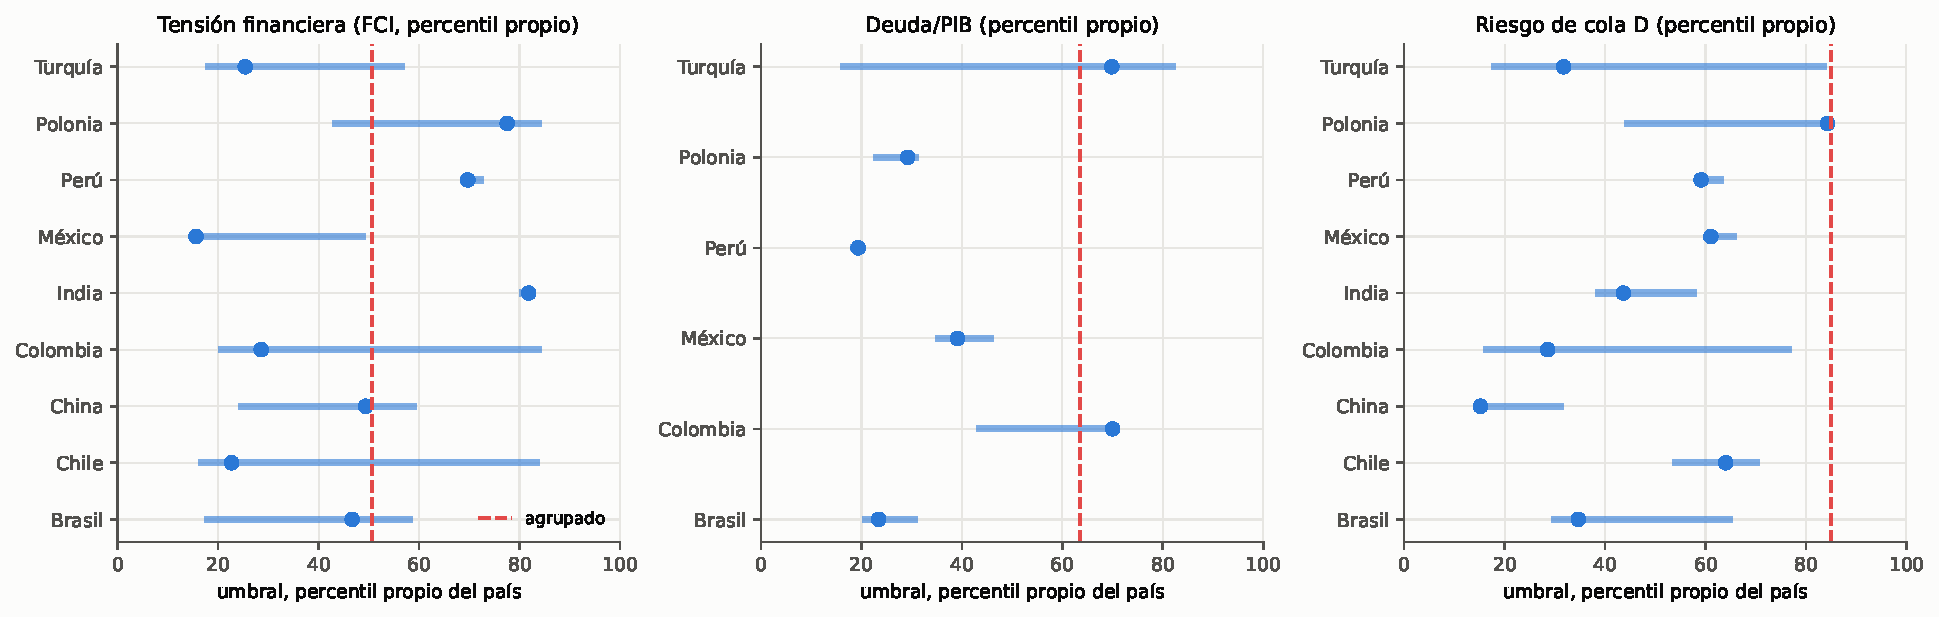
\includegraphics[width=\textwidth]{fig_umbrales_pais.pdf}
\caption[Umbrales por país frente al agrupado]{Umbrales estimados con la serie de cada economía (punto) y su intervalo al 90\,\% (barra), en el percentil propio de cada una, frente al umbral agrupado en percentiles (línea discontinua).}
\label{fig:umbrales-pais}
\end{figure}

Ninguna de las tres pruebas pasa la corrección de Holm (Tabla~\ref{tab:umbrales-prereg}). La transmisión no cambia de régimen con la tensión financiera doméstica de forma demostrable, y la potencia del contraste para un cambio de esa magnitud es de 68\%, de modo que un umbral grande se habría detectado con probabilidad razonable. Si algo cambia, es en la dirección contraria a la prevista: con más tensión, el riesgo de cola pesa menos en el spread, y con las medidas sistémicas de mercado ---MES y $\Delta$CoVaR, calculadas con los mismos bancos---, la fragilidad también pesa menos, esta vez con un umbral que el \textit{bootstrap} sí detecta. Es lo que cabe esperar si, en los episodios de tensión, el spread pasa a moverse con el ciclo financiero global, que explica la mayor parte de su varianza, y los riesgos domésticos pierden peso relativo. No es una prueba de ese mecanismo.

El umbral de deuda no se distingue del modelo lineal: la potencia es de solo 13\%, y la amplificación de la Sección~\ref{sec:resiliencia-prereg} se lee mejor como continua. Bajo un 25\% del PIB el riesgo de cola casi no pesa en el spread y sobre ese nivel pesa $0{,}067$, pero ese tramo bajo lo forman sobre todo China, Filipinas y parte de los trimestres de Perú e Indonesia: el umbral separa economías más que niveles de deuda dentro de cada una. Por país, el umbral de deuda es significativo en cuatro de seis, pero ninguna contiene el umbral agrupado en su intervalo, y en cinco de las seis un quiebre en una fecha ajusta igual o mejor: como la deuda cambia lento dentro de cada país, su umbral es un cambio en el tiempo, no un nivel de deuda.

\textbf{Agrupado frente a cada país.} La comparación decide, según la regla fijada en el preregistro, si un umbral puede servir como regla común. Para la tensión financiera, seis de nueve economías contienen el umbral agrupado y no se rechaza un umbral común ($p=0{,}34$), pero el umbral mismo no es significativo: no hay un umbral que compartir. Para la deuda y para el riesgo de cola se rechaza un umbral común ($p=0{,}06$ y $0{,}04$), y los umbrales de cada país, en su percentil propio, van del 19 al 70 y del 15 al 84 (Figura~\ref{fig:umbrales-pais}): no hay un umbral transferible entre economías. Al descontar el ciclo global con controles en lugar de los efectos de tiempo del panel, solo dos de nueve economías contienen el umbral de tensión agrupado.

\textbf{Alerta temprana.} Dentro de la muestra, el logit distingue los episodios de estrés soberano (AUROC de $0{,}71$), pero fuera de la muestra no supera al azar ($0{,}49$). Dentro de la muestra, la tensión financiera anticipa más episodios ($+0{,}82$ por desviación estándar), mientras que más fragilidad y más riesgo de cola anticipan \emph{menos} ($-0{,}35$ y $-0{,}51$): cuando esos riesgos ya están altos, el spread ya subió, y lo que sigue tiende a ser una corrección. Fuera de la muestra, la tensión financiera sola es la señal más informativa (AUROC de $0{,}58$), sin llegar a ser útil para un regulador. El semáforo preregistrado queda como ejercicio exploratorio: con los umbrales de pérdida mínima, casi todos los trimestres caen en ámbar. Las medidas macroprudenciales efectivas (base iMaPP del FMI) no se pudieron incorporar porque la base requiere acceso registrado.


\section{La cola alta del spread}
\label{sec:cuantilica}

La teoría ubica la amplificación en los estados adversos, y la regresión principal mide la media condicional del spread. Si la coincidencia de los dos riesgos solo importara cuando el spread ya está alto, la media podría esconderla. Por eso la especificación principal se estimó a lo largo de la distribución condicional del $\ln$ EMBI, de dos formas. La primera es la regresión cuantílica por momentos de \citet{MachadoSantosSilva2019}, que admite efectos fijos de país y de tiempo. La segunda es una regresión cuantílica con variables indicadoras de país y de tiempo, que no impone la estructura de localización y escala. Ambas se repiten con la distancia al incumplimiento en lugar de $\ln JLoss$. La inferencia remuestrea economías completas.

\begin{figure}[htbp]
\centering
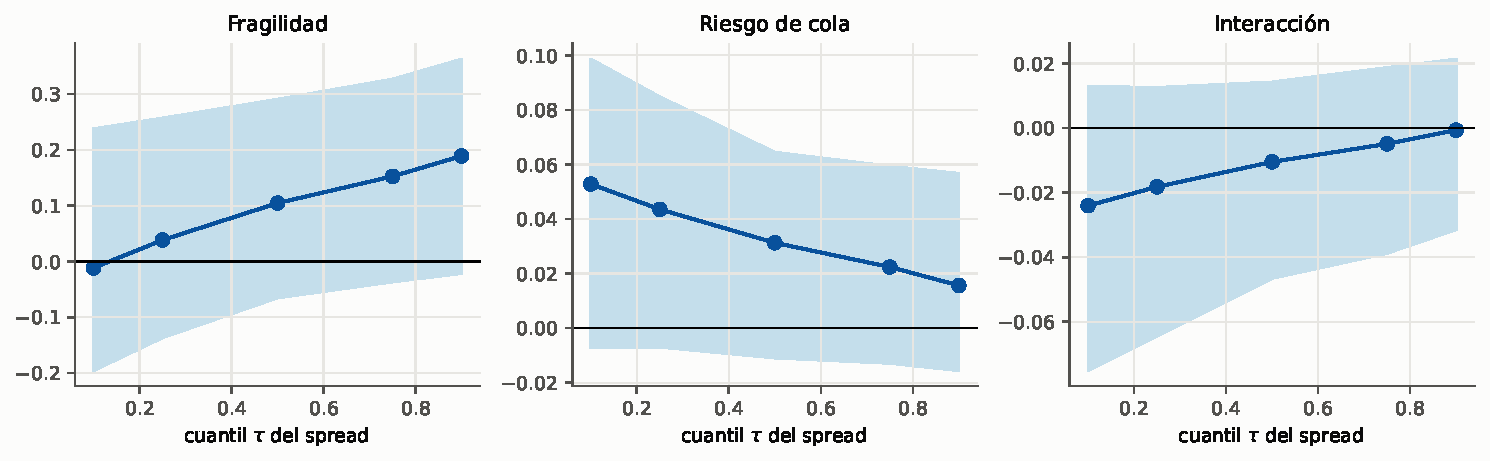
\includegraphics[width=\textwidth]{fig_cuantilica_lnlag.pdf}
\caption[Regresión cuantílica del spread]{Coeficientes de la especificación principal a lo largo de la distribución condicional del $\ln$ EMBI (regresión cuantílica por momentos con efectos fijos de país y de tiempo). Banda: intervalo al 95\% por \textit{bootstrap} de bloques de país (499 réplicas). Fuente: \texttt{p35\_cuantilica\_spread.py}.}
\label{fig:cuantilica}
\end{figure}

La interacción no aparece en la cola alta (Figura~\ref{fig:cuantilica}). Con la regresión por momentos crece de $-0{,}024$ en el cuantil 10 a $-0{,}001$ en el 90, y no es positiva ni significativa en ningún cuantil ($p\geq0{,}63$). Con las variables indicadoras oscila entre $-0{,}007$ y $+0{,}003$ ($p\geq0{,}86$). Con la distancia al incumplimiento llega a $+0{,}006$ en el cuantil 90 ($p=0{,}43$). Lo que sí cambia con el cuantil es el peso de cada riesgo por separado. La fragilidad importa más cuando el spread es alto: su elasticidad va de $-0{,}01$ en el cuantil 10 a $0{,}19$ en el 90, y con la distancia al incumplimiento es significativa en la mediana y en el cuantil 90 ($p=0{,}032$ y $0{,}024$). El riesgo de cola, en cambio, pesa algo más cuando el spread es bajo ($0{,}053$ en el cuantil 10 y $0{,}016$ en el 90), aunque sin significancia. La amplificación no está escondida en la cola del spread: lo que la cola alta muestra es una fragilidad bancaria que pesa más en los estados de estrés, por separado y no en combinación con el riesgo de cola.

\section{Una señal de valor relativo y la cola de los cambios del spread: pruebas preregistradas}
\label{sec:quant-prereg}

Un séptimo preregistro (\texttt{4\_Redaccion/preregistro\_quant.md}), escrito antes de construir cualquier retorno, lleva dos resultados de la tesis a las preguntas que haría quien gestiona un portafolio de deuda soberana emergente. La primera es si la precedencia mensual de la fragilidad (Sección~\ref{sec:mensual}) sirve para ordenar a los países según su retorno del mes siguiente (Q1). La segunda es si la simultaneidad de los dos riesgos, que no eleva el nivel del spread más que la suma, ensancha la distribución de sus cambios (Q3). Todo es mensual, de enero de 2015 en adelante (139 meses), y sin anticipación: el balance de los bancos se usa tres meses después de su fecha de cierre, el riesgo de cola es el del trimestre $q-2$ y el tercil alto de cada riesgo se define con la historia de cada país disponible hasta el mes anterior. El retorno de exceso se aproxima con una duración de siete años, $r\approx-7\,\Delta s+s/12$, porque no hay índices de retorno total por país en el repositorio, y cada operación paga la mitad de un \textit{bid-ask} de 15 puntos básicos de spread.

\begin{table}[htbp]
\centering
\small
\caption[Señal de valor relativo y cola de los cambios del spread]{Señal de valor relativo con la fragilidad (Q1) y cola de los cambios del spread bajo simultaneidad (Q3): pruebas preregistradas}
\label{tab:quant-prereg}
\begin{adjustbox}{max width=\linewidth}
\begin{tabular}{>{\raggedright\arraybackslash}p{4.6cm}>{\raggedright\arraybackslash}p{7.6cm}>{\raggedright\arraybackslash}p{2.6cm}}
\toprule
Hipótesis & Resultado & Holm \\
\midrule
Q1: cartera larga/corta por terciles del cambio mensual de la distancia al incumplimiento & Sharpe anual neto $-4{,}07$ (IC 90\,\%: $-4{,}93$ a $-3{,}17$); bruto $+0{,}01$ ($-0{,}44$ a $+0{,}43$); Fama--MacBeth, $t=-0{,}47$; rotación de 2,5 veces por mes & $1{,}00$: no pasa \\
\addlinespace
Q3-H1: escala de los cambios mensuales del spread (MMQR) & Fragilidad alta $+0{,}062$ ($p=0{,}005$); riesgo de cola alto $+0{,}019$ ($0{,}085$); su coincidencia $-0{,}046$ ($0{,}97$) & $1{,}00$: no pasa \\
\addlinespace
Q3-H2: VaR al 95\,\% fuera de la muestra & Condicional frente a EWMA: Diebold--Mariano $p=0{,}47$; cobertura condicional rechazada ($p=0{,}002$); el VaR histórico de 60 meses es el mejor de los tres & $1{,}00$: no pasa \\
\bottomrule
\end{tabular}
\end{adjustbox}
\par\smallskip\parbox{0.95\linewidth}{\footnotesize \textit{Nota:} 13 economías, 2015-01 a 2026-07 (139 meses; 10,8 países por mes en promedio). Q1: Sharpe con la prueba de Ledoit y Wolf (2008), \textit{bootstrap} circular por bloques de 6 meses (4\,999 réplicas). Q3-H1: regresión cuantílica por momentos \citep{MachadoSantosSilva2019}, con efectos de país y de mes en la localización y de país en la escala; $p$ unilateral por \textit{bootstrap} de países (999). Q3-H2: regresión cuantílica recursiva con indicadoras de país, frente a un VaR normal con volatilidad exponencial ($\lambda=0{,}97$); prueba de Diebold y Mariano (1995) sobre la pérdida cuantílica, y de Christoffersen (1998). Desviaciones declaradas: el EWMA y el VaR histórico no se interrumpen en los meses sin dato; el VaR se evalúa donde existen los tres pronósticos; con umbrales expansivos la coincidencia ocurre en el 37\,\% de la muestra. Fuente: \texttt{p60\_senal\_dd.py} y \texttt{p62\_cola\_cambios.py}.}
\end{table}

\textbf{La fragilidad no ordena los retornos entre países} (Tabla~\ref{tab:quant-prereg}). Bruto, el Sharpe de la cartera es nulo y la pendiente de Fama--MacBeth no se distingue de cero; neto de costos es fuertemente negativo, porque una cartera mensual rota dos veces y media su tamaño. El resultado es el mismo sin Turquía, con costos de 25 puntos básicos, con pesos por rango, a tres meses y por subperíodos. La precedencia mensual es una regularidad dentro de cada país, no una señal de valor relativo entre países.

\textbf{La coincidencia tampoco ensancha la cola de los cambios del spread.} Cada riesgo por separado ensancha la distribución de los cambios, la fragilidad con evidencia firme. Su coincidencia no la ensancha más: el término conjunto es negativo, también a tres meses, sin 2020--2021, con los terciles de toda la muestra y sin efectos de mes. Es el mismo patrón subaditivo de la interacción en el nivel (Sección~\ref{sec:aditivos}). Un VaR que usa los dos riesgos no pronostica mejor que uno de volatilidad exponencial y no pasa la prueba de cobertura condicional. Según las consecuencias fijadas, la conclusión ``simultaneidad sin amplificación'' queda igual, ahora también para la cola de los cambios, y la precedencia mensual de la fragilidad no cambia de grado.
